\chapter{Evaluación y Desempeño}


\section{Introducción}

Durante este capitulo nos dedicaremos a analizar el desempeño de nuestro agente. Para ello definiremos una serie de configuraciones, donde haremos variar los diferentes parámetros de ejecución y usaremos cada una de estas configuraciones sobre diferentes compañías para luego tratar de evaluar como dichos parámetros, afectan o no, en el desempeño del mismo. Lo interesante sera observar tanto los patrones de compra y venta ejecutados por el agente durante toda la simulación, como así también las ganancias obtenidas en cada configuración.

\section{Configuraciones}

La siguientes configuraciones serán ejecutas múltiples veces sobre diferente compañías. El objetivo principal de estas configuración es tratar de ver como se comporta el algortimo bajo diferentes seteos. 

En principio hemos considerado 3 configuración que según creemos una sera la  mas optima(moe), una intermedia(lenny) y por ultimo la que peor debería performar sera ralp, pues se acerca mucho a un agente que toma decisiones en forma aleatoria. 

\begin{table}[]
	\centering
	\caption{Configuraciones de los agentes}
	\label{my-label}
	\begin{tabular}{llll}
		Nombre                     & moe & lenny & ralph \\
		$\varepsilon$-greedy       & 0.1 & 0.3   & 1     \\
		learnig rate    $\alpha$   & 0.3 & 0.3   & 0.3   \\
		discount factor $\gamma$   & 0.8 & 0.5   & 0.1   \\
		mini batch                 & 50  & 100   & 10    \\
		memory replay      		   & 500 & 1000  & 5     \\
		hidden layers     		   & 4   & 8     & 2     \\
		neurons per layer  		   & 16  & 32    & 4    
	\end{tabular}
\end{table}

Ambas configuraciones se ejecutaran sobre dos compañías cuyos papeles tienen comportamientos completamente diferentes.
Una apple donde claramente puede verse que el valor de las acciones generalmente se encuentra dentro de un tendencias alcista durante los 10 años y la otra es microsoft la cual posee un comportamiento mas estable, con tramos alcistas, bajistas y tramos donde el papel lateraliza. Las decisiones del agente se mostraran con burbujas de color azul para las compras, y burbujas de color amarillo para las ventas, a media que transcurran los días, se irán marcado cada vela, con una burbuja indicando la acción, para poder simplificar la visualización del gráfico, hemos decidido, no marcar con ningún marcador, los decisiones de esperar.

\section{moe}

Estos son los resultados de la primera ejecución de moe sobre ambas compañías.

\begin{figure}[h!]
	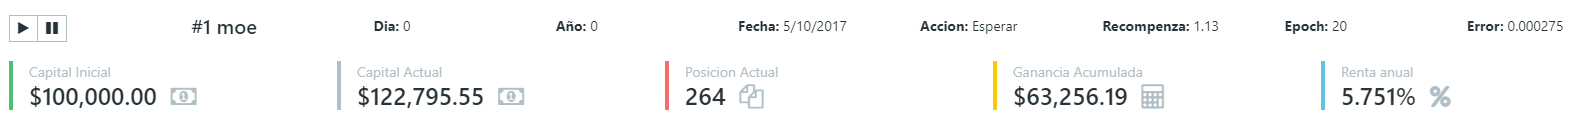
\includegraphics[scale=0.5]{imagenes/moe_appl_ex1_1_summary.png}
	\caption{Resultados de moe sobre apple}
\end{figure}

\begin{figure}[h!]
	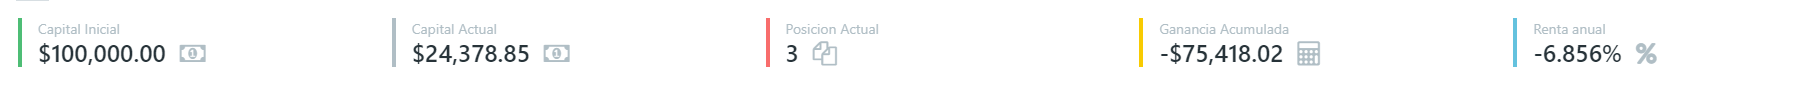
\includegraphics[scale=0.45]{imagenes/moe_msft_ex1_1_summary.png}
	\caption{Resultados de moe sobre microsoft}
\end{figure}

En este caso, el agente logro mejores resultados con apple, probablemente producto de la propia característica de un papel generalmente alcista.
Sin embargo, observemos que sucede durante los primeros días de la simulación.

\begin{figure}[h!]
	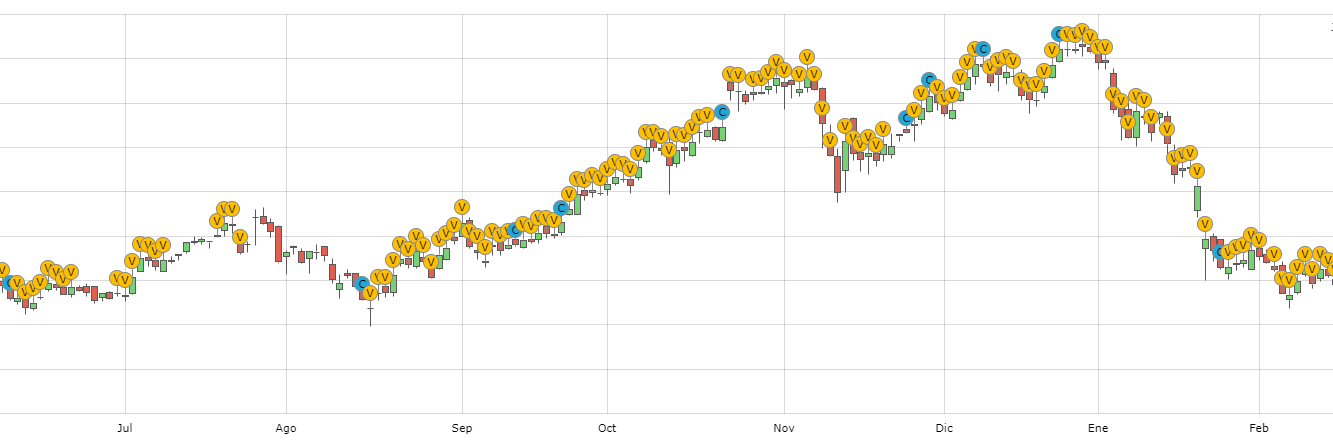
\includegraphics[scale=0.5]{imagenes/moe_appl_ex1_1.png}
	\caption{Primeros días de trading sobre apple}
\end{figure}

\begin{figure}[h!]
	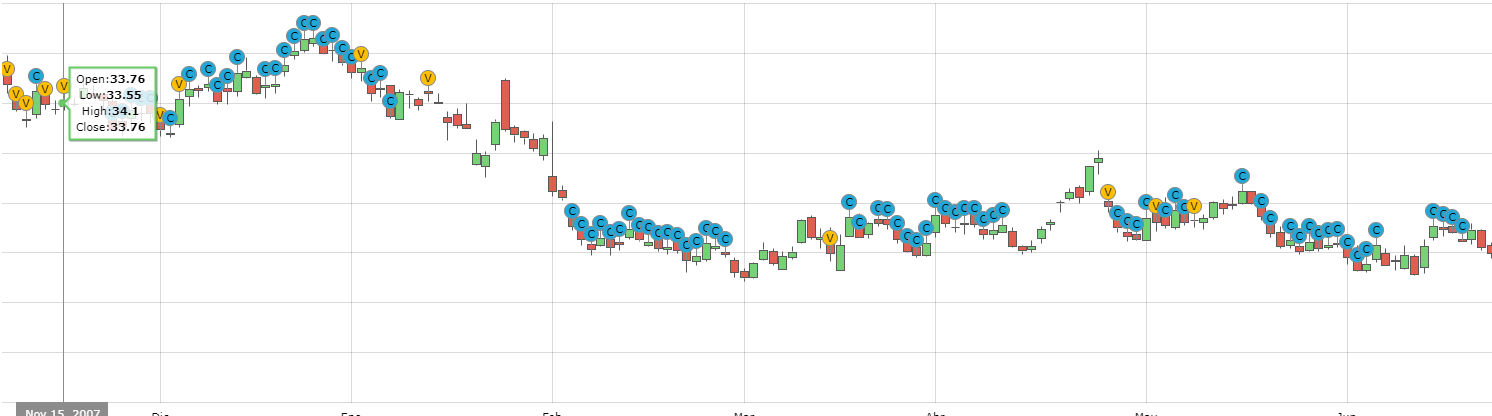
\includegraphics[scale=0.45]{imagenes/moe_msft_ex1_1.png}
	\caption{Primeros días de trading sobre microsoft}
\end{figure}

Claramente puede observarse que el agente se predispone mayoritariamente a realizar siempre la misma acción, en el primer caso decide vender, y en el segundo comprar.
Probablemente esto este determinado por la elección de la primera acción, pues sera la que en principio mas se repita, y de la que mayor conocimiento tiene sobre su recompenza futura. A media que vaya experimentado en forma aleatoria otras acciones, gracias a la policy $\varepsilon$-greedy, deberiamos esperar ver un cambio en el patrón de decisiones.
Veamos ahora que sucede con los últimos días de trading:

\begin{figure}[h!]
	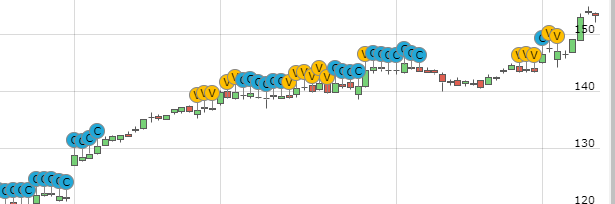
\includegraphics[scale=0.7]{imagenes/moe_appl_ex1_2.png}
	\caption{Últimos días de trading sobre apple}
\end{figure}

\begin{figure}[h!]
	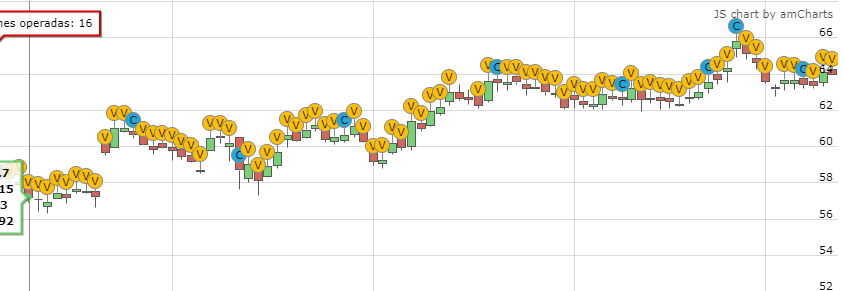
\includegraphics[scale=0.7]{imagenes/moe_msft_ex1_2.png}
	\caption{Últimos días de trading sobre microsoft}
\end{figure}

En ambos casos, puede observarse una mejoría, tal vez, en el caso de apple sea mas marcada, dado que hasta puede observarse que durante varios días, el agente solo decide esperar, y especular esperando que el precio suba para vender luego de varios días gran parte de sus acciones a un precio mucho mayor al que las compro.
Para el caso de microsoft, no es tan claro, pero sin embargo, puede verse que cada 4 o  5 días, el agente compra, para luego vender. Es importante notar aquí, que dado el esquema de entrada y salida que se decidió adoptar, los días en que compra, comprar mucho mas de lo que luego vende en los días siguientes.